% !TEX root = ../Dokumentation.tex
\subsection{Lenkung}

\textbf{Funktionsbeschrieb}
\\[0.2cm]
Die Lenkung ist eine Achsschenkellenkung. Sie wird heute in fast allen PKW, LKW, Omnibusse und sonstige Nutzfahrzeugen eingesetzt. Bei dieser Art der Lenkung befinden sich die Räder auf einzeln lenkbaren Achsschenkeln, die jeweils mit einem Spurstangenhebel versehen sind. Die Spurstangenhebel sind ungefähr senkrecht zur Vorderachse bzw. ungefähr parallel zur Längsachse des Fahrzeugs ausgerichtet und mittels einer Spurstange miteinander verbunden. Dadurch werden beide Räder gleichzeitig gelenkt.\\[0.2cm]
\textbf{Komponentenbeschrieb}
\\[0.2cm]
Mit einem Servomotor wird über eine Kegelradverbindung der Lenkschubhebel angetrieben. Dieser treibt wiederum die Spurstange an, welche die Bewegung Über die Spurstangenhebel an die Räder weitergibt.
\begin{figure}[H]%Position festigen
\centering
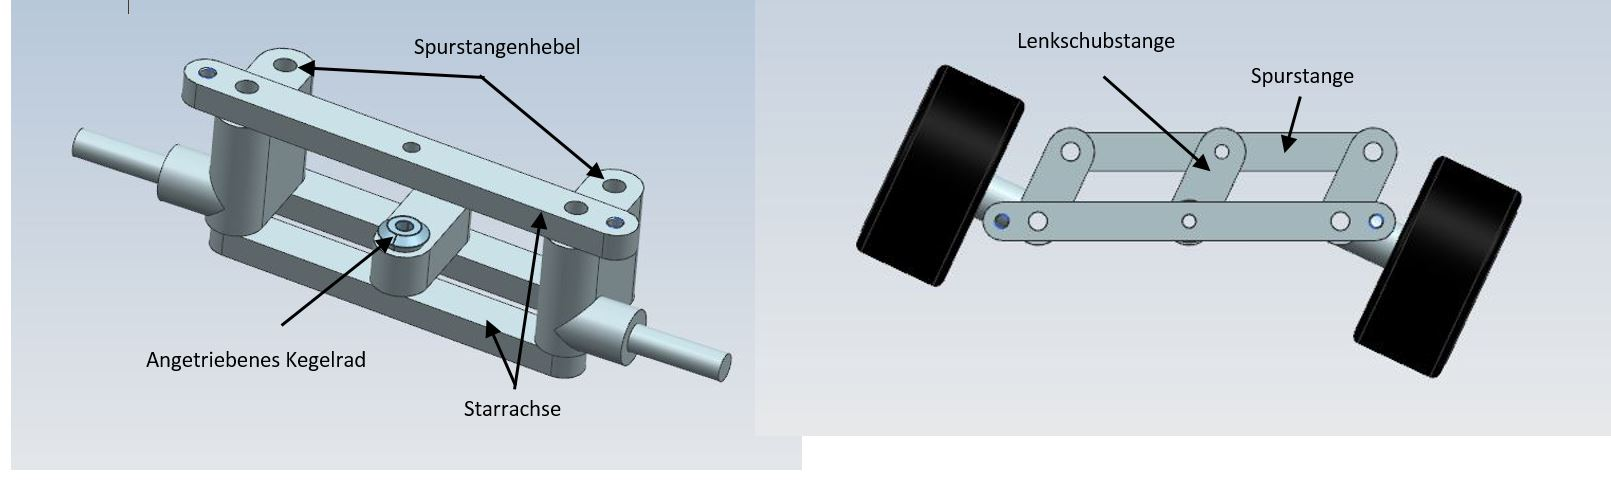
\includegraphics[width=1\textwidth]{03_Loesungskonzept/pictures/Achsschenkellenkung.JPG}
\caption{Konzept der Achsschenkellenkung}
\label{fig:activityRoute}
\end{figure}

\textbf{Begründung}\\[0.2cm]
Für die Bildverarbeitung ist das Lenken und konstante ausgleichen der Fahrbahn und Fahrtgeschwindigkeit mit zwei angetriebenen Rädern ein Nachteil. Von der Konstruktiven seit ist die Achsschenkellenkung im Vergleich zwar aufwändiger aber für die Aufgabenstellung besser geeignet. Da dass Ziel ist einen möglichst konstanten Abstand zum Trottoir der Fahrbahn zu halten, ist die Regelung einer Achsschenkellenkung einfacher. Weitere Gründe, welche für die Achsschenkellenkung sprechen wurden schon im Kapitel "Chassis" erläutert.
Die Begründung für die Wahl des Servomotors ist, dass die Lenkung keine 360° Bewegungen durchführen muss. Zudem ist die Drehzahl des Servos leicht zu steuern, ohne das zusätzlich eine Regelung eingebaut werden muss. 
